\addtocontents{toc}{\protect\vspace{\beforebibskip}} % Place slightly below the rest of the document content in the table

%************************************************
\chapter{Background}
\label{ch:background}
%************************************************

The scope of this internship concerns digital forensics, as it focuses on adapting an existing forensics platform into a collaborative client-server model.

In this chapter, a contextualization of digital forensics is given, an analysis of both \acrfull{tsk} \cite{sleuthkit} and Autopsy is made, and it's given a brief description and analysis of the existing forensic platform alternatives.

\section{Digital Forensics}

Forensic science \cite{nist} is the use of scientific methods or expertise to investigate crimes
or examine evidence that might be presented in a court of law.

The definition of digital forensics is directly related to the definition of
computer forensics, which is the collection, preservation, analysis,
and presentation \cite{daniels} of evidence stemming from digital sources for use in a legal matter
using investigative processes, tools, and practices.

Digital forensics \cite{nist2} is the application of computer technology to criminal cases where evidence
includes items that are created by digital systems.

Digital forensics is the field of forensic science that is concerned with retrieving,
storing and analysing electronic data that can be useful in criminal investigations.
This includes information from computers, hard drives, mobile phones and other data
storage devices.

Digital forensic investigators face challenges such as extracting data from damaged or destroyed
devices, locating individual items of evidence among vast quantities of data
and ensuring that their methods capture data reliably without altering it in any way.

Personal data should ultimately be attributable to an individual; however, making
that attribution can be difficult due to the presence or absence of individualized
user accounts, security to protect those user accounts, and the actual placement of a
person at the same location and time when the data is created.

\subsection{Digital Evidence}

Digital evidence is any type of digital data with incriminating characteristics,
which can result from any type of action preformed by a user, like transactions and
recordings.

Nowadays it's virtually impossible not to leave a digital track behind, since most
of us carry and use devices capable of connecting to the internet.

The explosion of social media sites has created a whole new area of electronic
evidence. Most people today are willing to share all kinds of information through
social media platforms.

In order for electronic data to become digital evidence, it must be stored and be recoverable
by a forensic examiner. One of the great challenges is not whether digital
evidence may exist, but where the evidence is stored, getting access to that storage,
and finally, recovering and processing that digital evidence for relevance within
a civil or criminal action.

The potential storage options for electronic evidence has shifted from being only contained locally
to being either located locally or remotely in what is called ``The Cloud`` \cite{cloud}. 

More and more everyday computing processes are moving to the Internet
where companies offer software as a service \cite{saas}. Software as a service means that
the customer no longer has to install software on their computer, allowing access to the software remotely,
and not storing any data locally.

%%TODO Comment about difficulty between retrieving local evidence and cloud stored evidence

\subsection{Processes and Procedures}

Digital forensics is the application of forensic science to electronic evidence in a
legal matter.

While there are many different subdisciplines and many types of devices, communication
and storage methods available, the basic principles of digital forensics
apply to all of them.

These principles encompass four areas:

\begin{enumerate}
\item Acquisition
\item Preservation
\item Analysis
\item Presentation.
\end{enumerate}

Each of these areas includes specific forensic processes and procedures.

\subsubsection*{Acquisition}

Acquisition is the process of collecting electronic data. Seizing a computer at a crime scene or
taking custody of a smartphone in a civil suit are examples of device acquisition, but the data 
must be extracted from these devices using specific procedures that equate to making a copy of
the storage devices, while following strict rules to ensure the integrity of all the extracted data.

Since acquisition is the first interaction between the investigators and the evidence,
it is the step where it's most likely to occur modifications of the contents of the seized devices,
because turning on the device or extracting the data without following the right procedures can alter
its contents irreversibly.

\subsubsection*{Preservation}

For evidence to be defendable in court, it must be preserved properly.
Preservation in the forensics context is the process of creating a chain of custody \cite{custody}
that begins before collecting the evidence and ends when the evidence is released.
Any interference in the chain of custody can lead to issues regarding the validity of the evidence.
Additionally, preservation includes maintaining the evidence in a safe environment, preventing
intentional destruction with malicious purpose or accidental modification by unqualified people.

A chain of custody log allows proving that the integrity of the evidence has been maintained from seizure
through presentation in court. It should contain entries for every time that a piece of evidence
has been touched, including collection, storage transport and any time the evidence is checked out for
handling by any personnel.

\subsubsection*{Analysis}

Analysis is the process of locating and categorizing items from evidence
that has been collected in a case. Each case is unique as the
circumstances surrounding each case can vary immensely, not only in the evidence being analysed, but also in the
approach used to perform the analysis. The analysis is the area where
the individual skills, tools used, and the training of the forensic examiner have
the greatest impact on the outcome of the examination. Considering that electronic evidence
appears in so many forms and comes from diverse locations and devices,
the training and experience of the examiner has a much greater impact
on the results of the examination.

Analysis of digital evidence is more than just determining whether a file exists on a hard drive, it involves finding out how
that file got on the hard drive, and if possible, who put the file on the hard drive.

\subsubsection*{Presentation}

Presentation of the examiner's findings is the last step in the process of forensic
analysis of electronic evidence. This includes not only the written findings or forensic
report, but also the creation of sworn statements, depositions of experts, and court testimony.
There are no exact rules or standards for reporting the results of an
examination. Each entity may have its own particular guidelines
for reporting. However, forensic examination reports should be written clearly, concisely,
and accurately, explaining what was examined, the tools used for the examination,
the procedures used by the examiner and the results of the examination.
The report should also include the collection methods used, including specific steps
taken to protect and preserve the original evidence and how the verification of the
evidence was performed.

\section{The Sleuth Kit}

\acrshort{tsk} is a library and collection of command line tools that allow the
investigation of disk images. The core functionality of \acrshort{tsk} allows volume and file system data analysis.
The plug-in framework allows incorporation of additional modules to analyse file contents
and build automated systems. The library can be incorporated into larger digital forensics tools and
the command line tools can be directly used to find evidence.

The original part of \acrshort{tsk} is a C library and collection of command line
file and volume system forensic analysis tools. The file system tools allow examining file systems
of a computer in a non-intrusive fashion. Because the tools do not rely on the operating system to process
the file systems, deleted and hidden content can be shown.

The volume system tools allow examination of the layout of disks
and other media. \acrshort{tsk} supports \acrshort{dos} partitions, \acrshort{bsd} partitions, Mac partitions, Sun slices, and 
GPT disks. With these tools, partition locations can be identified 
and extracted so that they can be analysed with file system analysis tools.

When performing a complete analysis of a system, command line 
tools can become tedious. Autopsy is a graphical interface to the tools in \acrshort{tsk}, 
which allows easier conduction of an investigation. Autopsy 
provides case management, image integrity, keyword searching and other automated
operations.

A complete analysis also requires more than just file and volume system analysis.
However, a single tool can't provide support for all file types and analysis 
techniques. The \acrshort{tsk} Framework allows tools to easily incorporate file analysis
modules that were written by other developers.

\acrshort{tsk} allows listing allocated and deleted \acrshort{ascii} and Unicode file names, can display the
details and contents of all \acrshort{ntfs} attributes, can display file system and meta-data structure details,
can create time lines of file activity, which can be imported into a spread sheet to create graphs and reports.
\acrshort{tsk} allows the lookup of file hashes in hash databases, it organizes files based on their type, and pages of
thumbnails can be made from graphic images to facilitate quick analysis.

\section{Autopsy}

Autopsy is a digital forensics platform and a graphical interface to \acrshort{tsk}
along with other digital forensics tools. It is used by law enforcement, military, 
and corporate examiners to investigate what happened on a computer. It can even 
be used by anyone to recover photos from a camera's memory card.

Autopsy was designed to be intuitive out of the box. Installation is easy and
wizards guide the user through every step. All results are shown in a single tree, as can be seen in Figure \ref{fig:tree}.

\begin{figure}[ht]
 \centering
 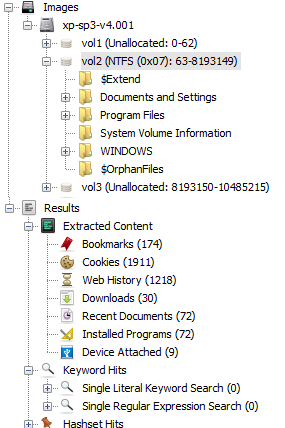
\includegraphics[width=0.5\linewidth]{imgs/tree.png}
 \caption{Autopsy's Explorer Tree}
 \label{fig:tree}
\end{figure}

Autopsy was designed to be an end-to-end platform with modules that come with
it out of the box and others that are available from third-parties. An overview of Autopsy's modules can be found in Table \ref{tab:autopsyModules}.

\begin{table}[!ht]
  \begin{tabularx}{\textwidth}{@{}|c| *1{>{\centering\arraybackslash}X}@{}|}
    \hline
    \textbf{Name} & \textbf{Description} \\
    \hline\hline
    Timeline Analysis & Advanced graphical event viewing interface \\
    \hline
    Hash Filtering & Flag known bad files and ignore known good \\
    \hline
    Keyword Search & Indexed keyword search to find files that mention relevant terms \\
    \hline
    Web Artifacts & Extract history, bookmarks, and cookies from Firefox, Chrome, Internet Explorer and Microsoft Edge \\
    \hline
    Data Carving & Recover deleted files from unallocated space \\
    \hline
    Multimedia & Extract \acrshort{exif} metadata from pictures and videos and display these files \\
    \hline
    Indicators of Compromise & Scan a computer using \acrshort{stix} \\
    \hline
  \end{tabularx}
    \caption{Autopsy's Modules}
  \label{tab:autopsyModules}
\end{table}

Autopsy runs background tasks in parallel using multiple cores and provides results as soon as they are found.

Autopsy is free and open source, allowing for cost-effective digital forensics analysis and community contributions.

\section{Related Software}

There are plenty of alternatives to Autopsy in the form of digital forensic analysis platforms, but the ones with most recognition work on a software as a service model, 
without providing a free trial, so even though it wasn't possible to test them, they were analysed based on the available information.

\subsection{Nuix Lab}

Nuix Lab \cite{nuix} allows investigators to work on large investigations.
It can be used for local or small regional forensic labs handling high data volume, variety, and 
complex digital evidence and looking to build or upgrade a dedicated digital forensics facility.

The core technologies of the Nuix Lab, Nuix Workstation and Nuix Investigate, give digital forensic technicians and case investigators 
different viewpoints into the same case data. Investigators can collaborate on 
the same data at the same time by using browser based tools.

The Implementation of Elasticsearch \cite{elasticsearch} as a data store for the Nuix Lab boosts evidence processing, investigation, and intelligence capabilities. 

Nuix Lab also claims to contain powerful artificial intelligence, machine learning, and analytics which should make it stand out from the competition. 

\subsection{EnCase Forensic}

EnCase Forensic \cite{encase} enables searching, identifying, and prioritizing potential evidence, in computers and mobile devices, to determine whether 
further investigation is warranted.

It can collect from a wide variety of operating and file systems, including over 25 types of mobile devices, and parses the most popular mobile apps across iOS, Android, and Blackberry devices.
Has strong decryption capabilities, allowing identification and unlocking password-protected files, and contains a custom indexing engine.

EnCase Forensic provides a wide range of capabilities that enable performing deep forensic analysis as well as fast triage analysis from the same solution, and provides a flexible
reporting framework that empowers tailoring case reports to meet specific needs.

\subsection{Forensics Toolkit}

\acrfull{ftk} \cite{ftk} is an award-winning, court-cited digital investigations solution. 

It locates evidence, collects and analyses any digital device or system producing, transmitting or 
storing data by using a single application for multiple devices.

All digital evidence is stored in one case database. It reduces the time, cost and complexity of creating multiple datasets, and there is continuous data transfer between AccessData's forensic 
and e-discovery solutions, allowing for collaboration between all parties working on the case. 

\acrshort{ftk} allows users to create images, process a wide range of data types, analyse the registry, crack passwords and build reports. 

\acrshort{ftk} allows collaboration, contains indexed searches, constructs timelines and other graphical assets, categorizes all the extracted artifacts and also contains malware identification modules.

\section{Comparison}

A comparison of the features offered by each software is presented in Table \ref{tab:comparison}.

\begin{table}[ht]
  \begin{tabularx}{\textwidth}{|c|c|c|c|c|}
    \hline
    \textbf{Feature} & \textbf{Autopsy} & \textbf{Nuix} & \textbf{Encase} & \textbf{\acrshort{ftk}} \\
    \hline\hline
    Collaboration & \cmark & \cmark & \cmark & \cmark \\
    \hline
    Web Based Interface & \xmark & \cmark & \xmark & \xmark \\
    \hline
    Indexed Searches & \cmark & \cmark & \cmark & \cmark \\
    \hline
    Decryption & \xmark & \xmark & \cmark & \cmark \\
    \hline
    Artificial Intelligence & \xmark & \cmark & \cmark & \xmark \\
    \hline
    Malware Analysis & \xmark & \xmark & \xmark & \cmark \\
    \hline
    Report Generation & \cmark & \cmark & \cmark & \cmark \\
    \hline
    Free and Open Source & \cmark & \xmark & \xmark & \xmark \\
    \hline
    Modular Plugins & \cmark & \xmark & \xmark & \xmark \\
    \hline
  \end{tabularx}
    \caption{Software Comparison}
  \label{tab:comparison}
\end{table}

Every software listed has its pros and cons; Autopsy mainly benefits from being free and open source, and allowing the development of modular plugins, while the other options seem to try to offer a very complete package out of the box.

Any of these software options seem viable for any kind of digital forensics investigation, and as a digital forensics firm, the teams should first test all these available options and chose the ones that best suit their needs.
